%%%%%%%%%%%%%%%%%%%%%%%%%%%%%%%%%%%%%%%%%%%%%%%%%%%%%%%%%%%%%%%%%%%%%%%
% BAB 5 IMPLEMENTASI DAN PENGUJIAN
%%%%%%%%%%%%%%%%%%%%%%%%%%%%%%%%%%%%%%%%%%%%%%%%%%%%%%%%%%%%%%%%%%%%%%%
%
%
% model h5 diubah dulu ke tflite
% untuk inferensi, dibuat aplikasi web menggunakan flask
% aplikasi web ini bisa diakses oleh user
% user mengupload file rekam ecg kemudian nanti hasilnya akan ditampilkan
% aplikasinya dideploy pada raspi5 dan intel nuc
% nanti akan diuji performanya dengan cara menghitung waktu inferensi dan memory usage
% pengujian inferensinya dilakukan dengan menggunakan dataset ecg dengan panjang 10 detik sejumlah 5 kali, panjang 1 menit sejumlah 5 kali, dan panjang 10 menit sejumlah 5 kali
% pengujian memory dilakukan dengan memantau memory usage maksimum yang digunakan oleh aplikasi ketika melakukan inferensi
% pengujian waktu inferensi dilakukan dengan memantau waktu yang dibutuhkan oleh aplikasi untuk melakukan inferensi mulai dari aplikasi menerima file rekam ecg hingga menghasilkan output
% dari masing-masing 5 kali pengujian, diambil rata-rata waktu inferensi dan memory usage
% 
%
%

\mychapter{5}{BAB 5 IMPLEMENTASI DAN PENGUJIAN}
Pada bab ini akan dijelaskan implementasi dari model yang telah dilatih sebelumnya serta pengujian performa inferensi model yang dilakukan pada perangkat tepi.
Terdapat tiga tahapan yang dilakukan, yaitu konversi model dari format H5 ke TFLite, implementasi aplikasi web untuk melakukan inferensi, dan pengujian performa inferensi pada perangkat tepi.
% Tahapan implementasi meliputi konversi model dari format H5 ke TFLite, pembuatan aplikasi web untuk melakukan inferensi, dan pengujian performa inferensi pada perangkat tepi.

\section{Konversi Model ke TFLite}
% from tensorflow.keras.models import load_model
% import tensorflow as tf
% for model_path in model_list:
%   model = load_model(model_path)
%   converter = tf.lite.TFLiteConverter.from_keras_model(model)
%   converter._experimental_default_to_single_batch_in_tensor_list_ops = True
%   converter.optimizations = [tf.lite.Optimize.DEFAULT]
%   tflite_model = converter.convert()
%   open(model_path.replace('.h5', '.tflite'), 'wb').write(tflite_model)

Model yang telah dilatih dengan menggunakan TensorFlow sebelumnya memiliki format H5.
Format H5 merupakan format yang belum dioptimasi sehingga memiliki ukuran yang besar dan tidak efisien untuk dijalankan pada perangkat yang memiliki keterbatasan sumber daya.
Untuk itu, model yang telah dilatih perlu
diubah ke format TensorFlow Lite (TFLite) agar dapat dijalankan pada perangkat yang memiliki keterbatasan sumber daya.
TFLite merupakan format yang dioptimasi untuk dijalankan pada perangkat yang memiliki keterbatasan sumber daya.
Selain itu, TFLite juga memiliki ukuran yang lebih kecil dan dependensi yang lebih sedikit dibandingkan dengan model TensorFlow biasa.

% dont include code in the main text, put it in the appendix
Untuk mengubah model dari format H5 ke TFLite, digunakan TFLiteConverter yang disediakan oleh TensorFlow.
TFLiteConverter adalah sebuah API yang disediakan oleh TensorFlow untuk mengubah model TensorFlow ke format TFLite.
Pada proses konversi, dilakukan optimisasi dengan cara kuantisasi.
Kuantisasi adalah teknik yang digunakan untuk mengurangi presisi dari angka yang digunakan untuk merepresentasikan parameter dari model.
Dengan mengurangi presisi, ukuran model dapat dikurangi dan dapat meningkatkan performa dan efisiensi inferensi model.
% Kuantisasi yang digunakan yaitu Dynamic range quantization. Dynamic range quantization is a recommended starting point because it provides reduced memory usage and faster computation without having to provide a representative dataset for calibration. 
Kuantisasi yang digunakan adalah \textit{Dynamic range quantization}.
\textit{Dynamic range quantization} mampu mengurangi penggunaan memori dan meningkatkan kecepatan komputasi tanpa perlu menyediakan dataset representatif untuk kalibrasi.

% Secara default, konversi model lstm ke format tflite memiliki dynamic batch size dan memerlukan ops default tensorflow, sehingga memerlukan dependensi tensorflow untuk menggunakannya. Agar dapat digunakan hanya dengan dependensi tflite runtime make perlu untuk mengubah batch size menjadi = 1.
Ketika model LSTM dikonversi ke format TFLite, model tersebut menggunakan
% dynamic batch size 
ukuran batch yang dinamis
% dan memerlukan \textit{ops} bawaan TensorFlow.
% gunakan bahasa indonesia sederhana, jangan istilah
dan memerlukan operasi bawaan TensorFlow.
Hal ini menyebabkan model TFLite tersebut memerlukan dependensi TensorFlow untuk dijalankan.
Untuk menghindari dependensi TensorFlow, batch size pada model TFLite perlu diubah menjadi 1.
Dengan mengubah batch size menjadi 1, model TFLite dapat dijalankan tanpa memerlukan dependensi TensorFlow.

% --- tabel komparasi ukuuran model sebelum dan sesudah konversi ---
% lstm-512 14.3M 1.2M
% lstm-256 3.6M 318.5k
% bi-lstm 8.0M 694.4k
% lstm-fcn 3.4M 299.4k

\begin{table}[H]
  \centering
  \caption{Perbandingan ukuran model sebelum dan sesudah konversi}
  \label{tab:ukuran-model}
  \begin{tabularx}{0.8\textwidth} {
    | >{\centering\arraybackslash}X
    | >{\centering\arraybackslash}X
    | >{\centering\arraybackslash}X | }
    \hline
    \textbf{Model} & \textbf{Ukuran (H5)} & \textbf{Ukuran (TFLite)} \\
    \hline
    LSTM-512 & 14,3 MB & 1,2 MB \\
    \hline
    LSTM-256 & 3,6 MB & 318,5 KB \\
    \hline
    Bi-LSTM & 8,0 MB & 694,4 KB \\
    \hline
    LSTM-FCN & 3,4 MB & 299,4 KB \\
    \hline
  \end{tabularx}
\end{table}

Tabel \ref{tab:ukuran-model} menunjukkan perbandingan ukuran file model sebelum dan sesudah konversi ke format TFLite.
Dari tabel tersebut, dapat dilihat bahwa ukuran model setelah dikonversi ke format TFLite lebih kecil dibandingkan dengan ukuran model sebelum dikonversi.
Ukuran model berkurang hingga 90\% setelah dikonversi ke format TFLite.
Ukuran model yang lebih kecil ini dapat mengurangi penyimpanan yang dibutuhkan untuk menyimpan model.
Selain itu, ukuran model yang lebih kecil juga dapat 
mengurangi waktu yang dibutuhkan untuk memuat model ke memori dan
mengurangi penggunaan memori ketika melakukan inferensi.



\section{Implementasi Aplikasi Web}
% user -> upload -> preprocess -> rpeak detection -> feature extraction -> predict -> result

Untuk melakukan inferensi model, dibuat sebuah aplikasi berbasis web yang dapat diakses oleh pengguna.
Aplikasi web ini dibuat menggunakan Flask.
% Alur kerja aplikasi web ditunjukkan pada Gambar \ref{fig:alur-kerja-aplikasi-web}.
\textit{Sequence diagram} dari aplikasi web ditunjukkan pada Gambar \ref{fig:alur-kerja-aplikasi-web}.
Pengguna dapat mengunggah file rekaman ECG pada aplikasi web.
Setelah pengguna mengunggah file rekaman ECG, aplikasi web akan melakukan inferensi menggunakan model TFLite yang telah dikonversi sebelumnya.
Hasil prediksi kemudian akan ditampilkan pada pengguna.

\begin{figure}[H]
  \centering
  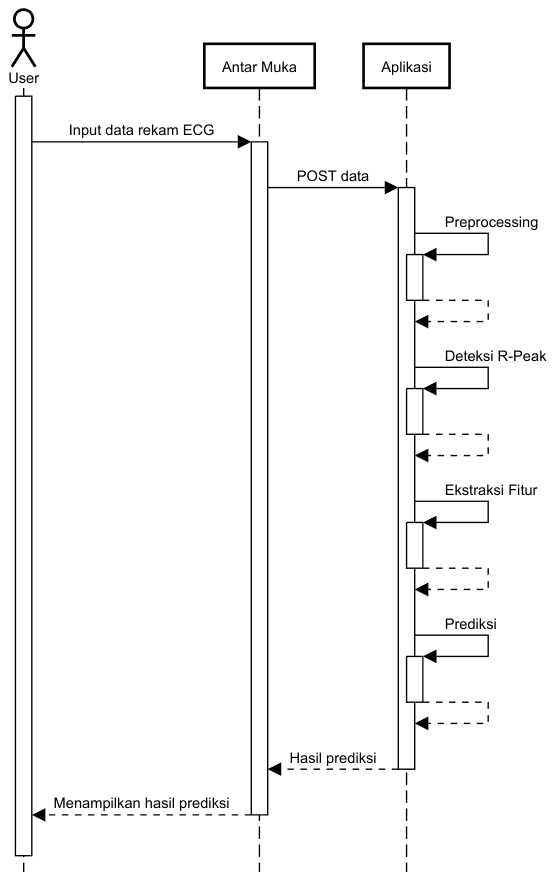
\includegraphics[width=0.6\textwidth]{img/sequence.png}
  \caption{\textit{Sequence diagram} aplikasi web}
  \label{fig:alur-kerja-aplikasi-web}
\end{figure}

% Gambar \ref{fig:aplikasi-web} menunjukkan tampilan aplikasi web yang dibuat.
Tampilan aplikasi web yang dibuat ditunjukkan pada Gambar \ref{fig:aplikasi-web}.
% Pengguna dapat mengunggah file rekaman ECG pada aplikasi web dan memilih model yang akan digunakan untuk melakukan prediksi.
% Tampilan aplikasi web terdiri dari beberapa bagian, yaitu bagian form input yang digunakan untuk mengunggah file rekaman ECG serta memilih model yang akan digunakan untuk melakukan prediksi, dan output yang akan menampilkan hasil prediksi yang terdiri dari diagram batang jumlah masing-masing kelas, tampilan sinyal ecg yang, dan tampilan sinyal pada masing-masing detak jantung.
Tampilan aplikasi web terdiri dari dua bagian utama, yaitu bagian input pengguna dan bagian output hasil prediksi.
Pada bagian input pengguna, pengguna dapat mengunggah file rekaman ECG dan memilih model yang akan digunakan untuk melakukan prediksi.
Pada bagian output hasil prediksi, terdapat tampilan output hasil prediksi yang terdiri dari diagram batang masing-masing kelas, tampilan keseluruhan sinyal ECG, dan tampilan sinyal ecg pada masing-masing detak jantung.
% Pengguna dapat mengunggah file rekaman ECG pada aplikasi web.
% Pengguna juga dapat memilih model yang akan digunakan untuk melakukan prediksi.
% Pengguna kemudian dapat menekan tombol \textit{Predict} untuk memulai proses prediksi.
Pada aplikasi web ini, pengguna dapat memilih model yang akan digunakan untuk melakukan prediksi.
Setelah pengguna mengunggah file rekaman ECG dan memilih model, pengguna dapat menekan tombol \textit{Predict} untuk memulai proses prediksi.
Setelah proses prediksi selesai, hasil prediksi akan ditampilkan pada pengguna.

% --- gambar ui aplikasi web ---
\begin{figure}[H]
  \centering
  % 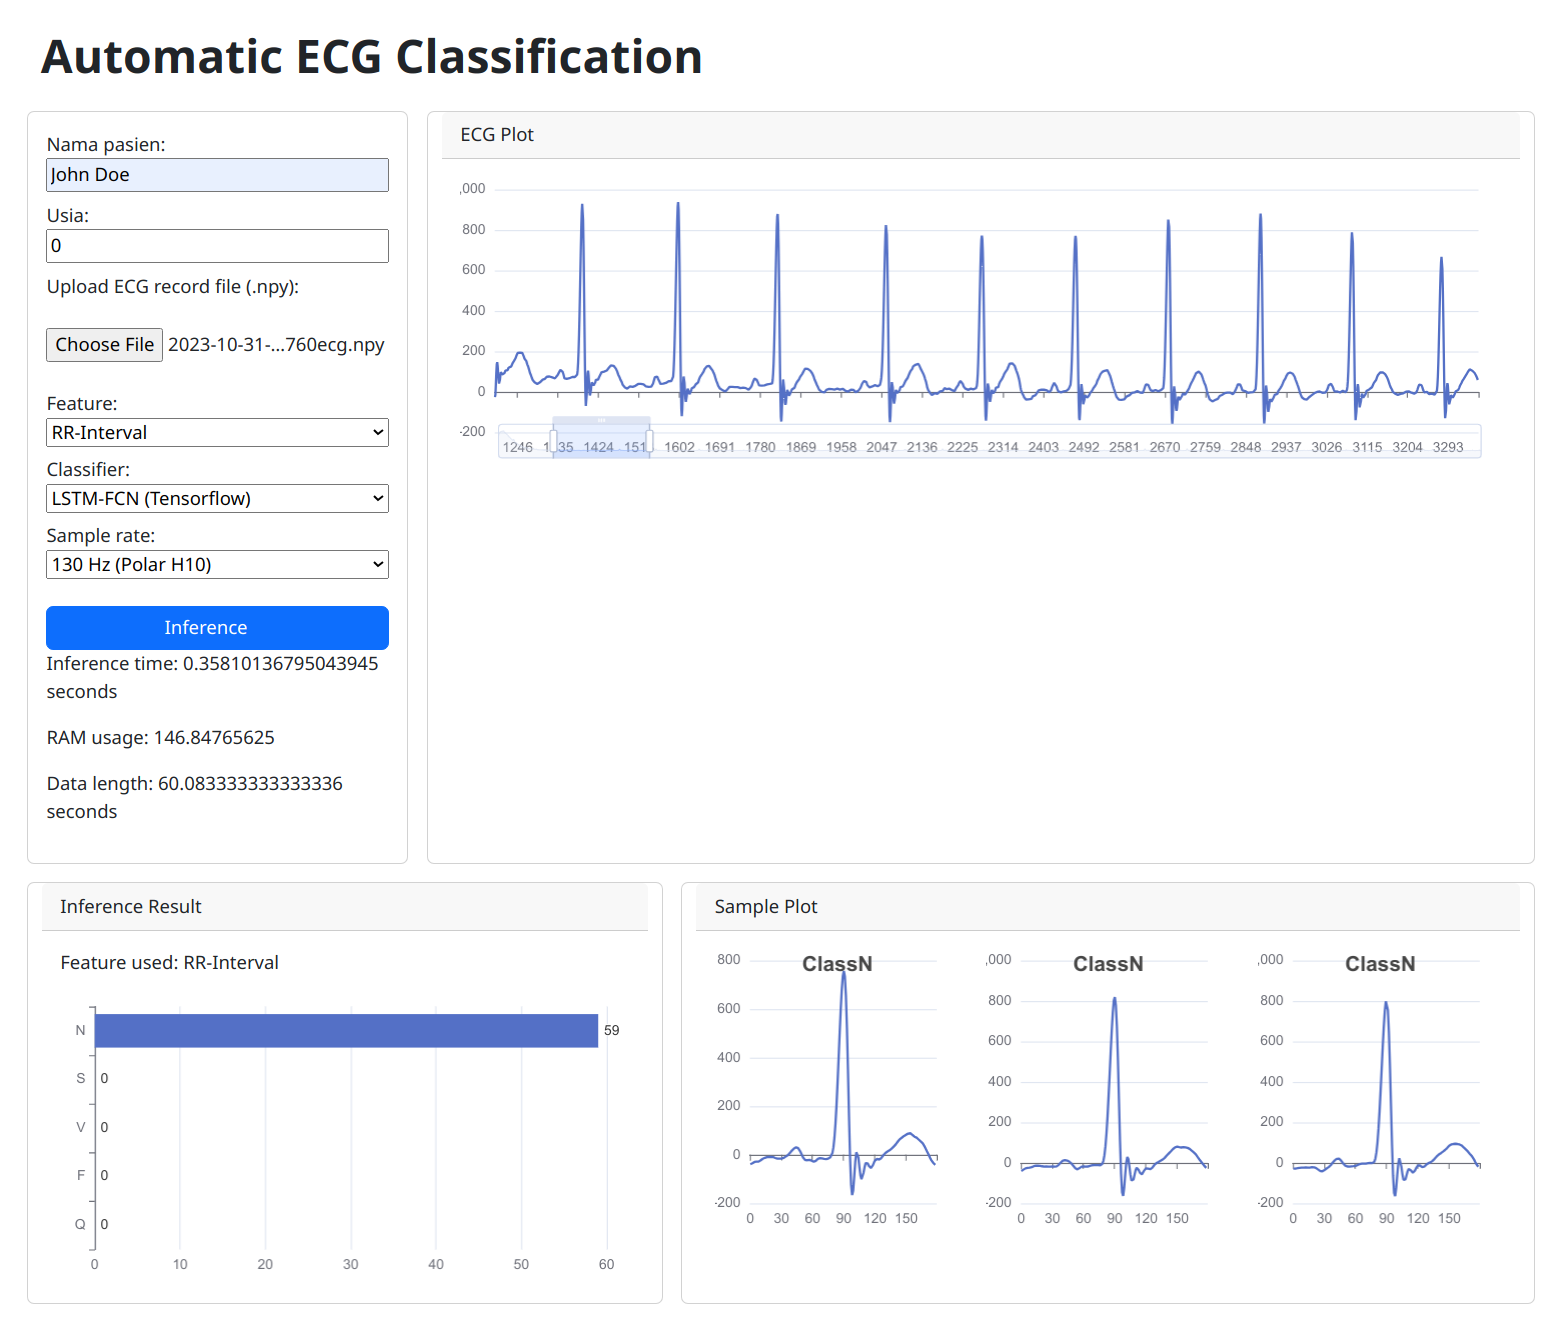
\includegraphics[width=0.8\textwidth]{img/tampilan-web.png}
  \fbox{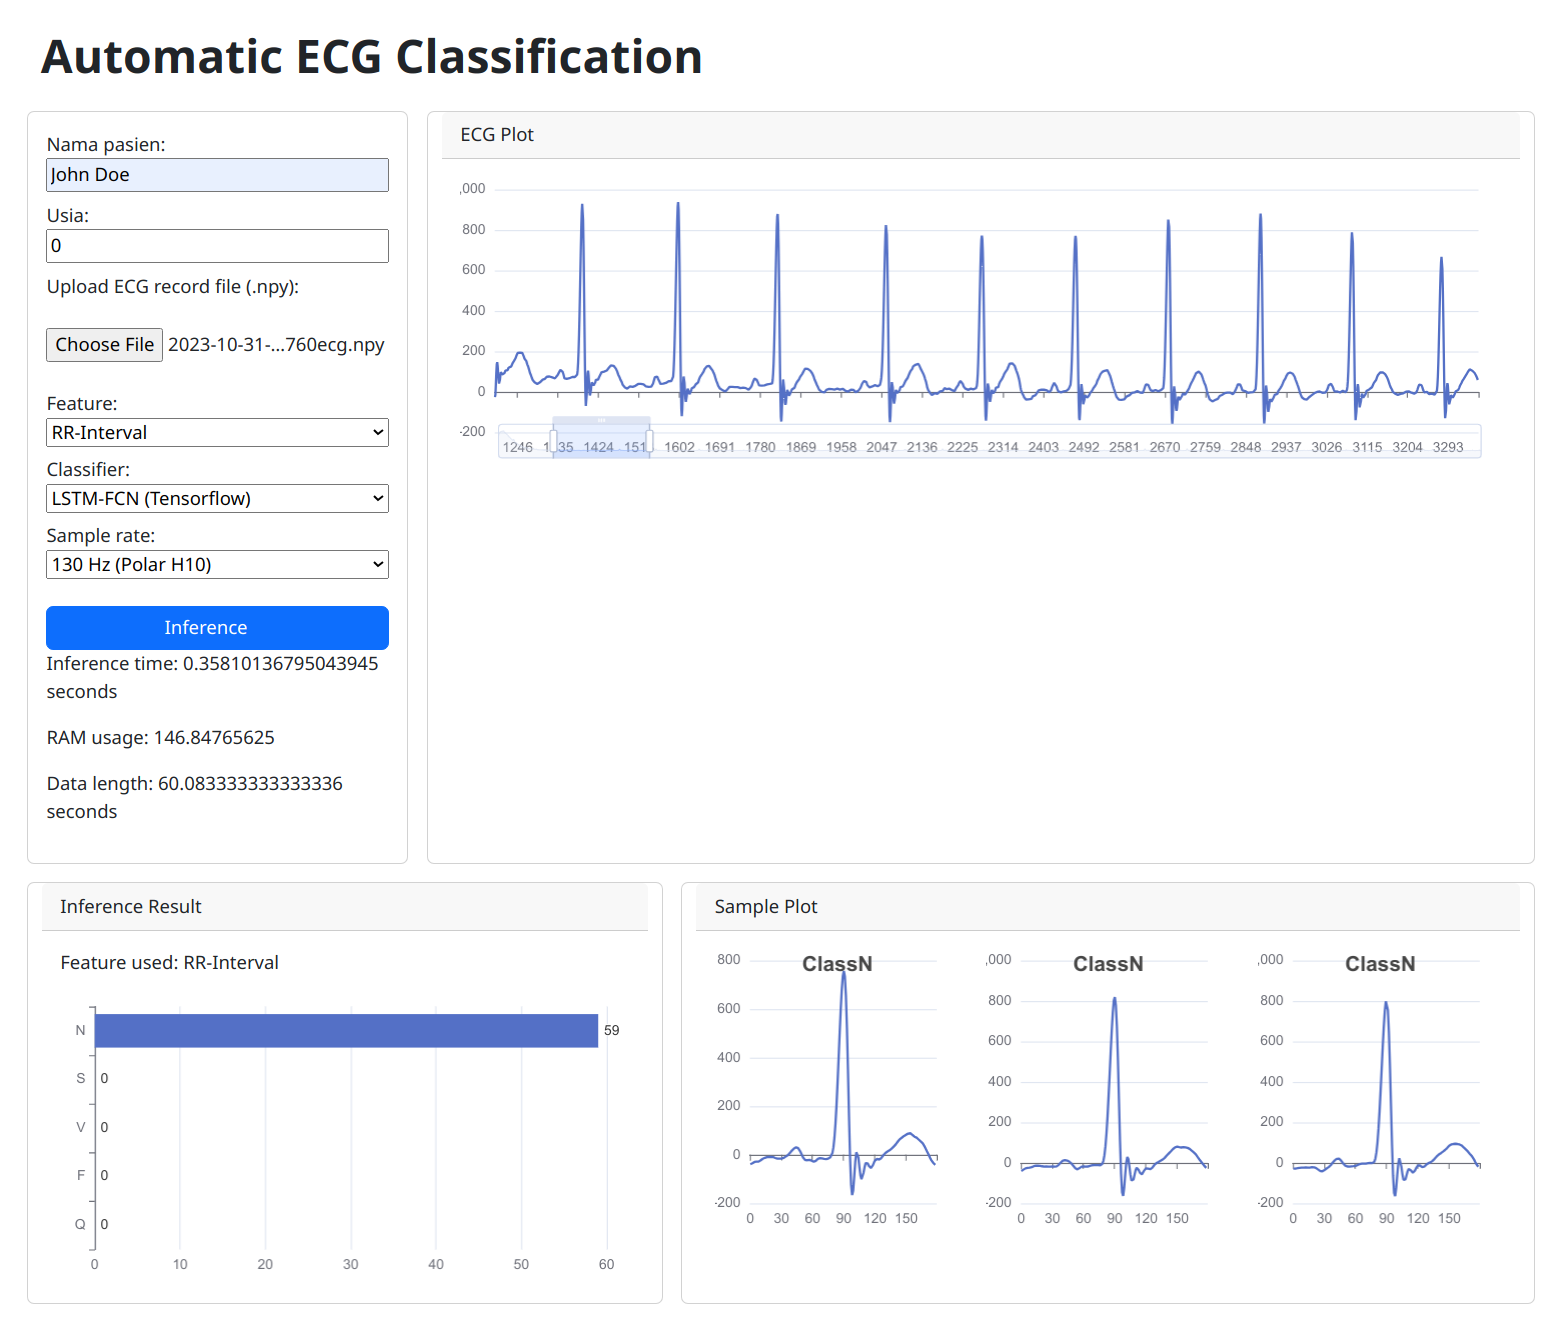
\includegraphics[width=0.9\textwidth]{img/tampilan-web.png}}
  \caption{Tampilan aplikasi web}
  \label{fig:aplikasi-web}
\end{figure}

% Proses inferensi terdiri dari beberapa tahap, yaitu \textit{preprocessing}, deteksi R-peak, ekstraksi fitur, dan prediksi.
Pada proses inferensi, terdapat beberapa tahapan yang dilakukan, yaitu \textit{preprocessing}, deteksi R-peak, ekstraksi fitur, dan prediksi.
% Sebelum data ECG dapat digunakan untuk melakukan prediksi, data ECG perlu diproses terlebih dahulu.
\textit{Preprocessing} dilakukan untuk membersihkan data dari gangguan dan mempersiapkan data untuk tahap selanjutnya.
Proses \textit{preprocessing} terdiri dari resampling, penghapusan \textit{noise} frekuensi tinggi menggunakan \textit{wavelet denoising}, penghapusan \textit{baseline wander}, dan normalisasi menggunakan \textit{z-score normalization}.
% --- pindahan dari bab 4 ---

% trained on 360hz mitboh but will be tested on 130hz polar h10
Data ECG yang akan digunakan untuk melakukan pengujian merupakan data yang direkam menggunakan perangkat Polar H10.
Data ECG yang direkam menggunakan perangkat Polar H10 tersebut memiliki frekuensi sampel 130 Hz, sedangkan dataset yang digunakan untuk melatih model memiliki frekuensi sampel 360 Hz.
% Sementara itu, model yang telah dilatih sebelumnya menggunakan dataset yang memiliki frekuensi sampel 360 Hz.
Oleh karena itu, data rekaman ECG perlu diubah ke dalam frekuensi sampel 360 Hz agar dapat digunakan untuk melakukan prediksi menggunakan model yang telah dilatih sebelumnya.
% using scipy resample
Data rekaman ECG diubah ke dalam frekuensi sampel 360 Hz menggunakan metode \textit{resampling}.
\textit{Resampling} dilakukan dengan menggunakan bantuan fungsi \textit{resample} yang disediakan oleh pustaka SciPy.
% dengan jumlah target sampel yang dihitung menggunakan persamaan \ref{eq:resample}
% \begin{equation}
%     N_{\text{target}} = \frac{360}{130} \times N_{\text{asal}}
%     \label{eq:resample}
% \end{equation}
% dengan $N_{\text{target}}$ dan $N_{\text{asal}}$ masing-masing menunjukkan jumlah sampel target dan jumlah sampel asal.


Selama proses pengambilan data, sinyal ECG rentan terhadap \textit{noise} berfrekuensi tinggi.
Frekuensi tinggi pada data ECG dianggap sebagai \textit{noise} yang dapat mengganggu proses klasifikasi detak jantung.
Pada penelitian ini, \textit{noise} berfrekuensi tinggi dihilangkan dengan menggunakan metode \textit{wavelet denoise}.
\textit{Wavelet denoise} menghilangkan \textit{noise} pada sinyal maupun gambar dengan menggunakan \textit{wavelet transform}.
\textit{Wavelet transform} memungkinkan sinyal untuk dipecah menjadi beberapa bagian frekuensi yang berbeda, sehingga memungkinkan penghilangan \textit{noise} pada frekuensi tertentu.
Metode \textit{wavelet denoise} yang digunakan pada penelitian ini adalah \textit{VisuShrink} dengan mode \textit{soft thresholding}, dan menggunakan \textit{wavelet} Daubechies 8 (db8) dengan 10 level \textit{wavelet decomposition}.

% --- dijelaskan lebih detail? ---

% Sinyal ECG diubah ke dalam domain \textit{wavelet} dengan menggunakan \textit{wavelet transform} Daubechies 8 (db8) dengan 10 level \textit{wavelet decomposition}.
% \textit{Noise} pada sinyal ECG kemudian dapat dihilangkan dengan mengurangi koefisien \textit{wavelet} yang memiliki nilai di bawah ambang batas tertentu.

%
% Setelah menghilangkan \textit{noise} berfrekuensi tinggi, tahap selanjutnya adalah menghilangkan \textit{baseline wander} (BW).
% elaborate
Selain \textit{noise} berfrekuensi tinggi, sinyal ECG juga rentan terhadap \textit{baseline wander}.
\textit{Baseline wander} (BW) merupakan \textit{noise} berfrekuensi rendah yang terdapat pada ECG.
BW dapat disebabkan oleh beberapa faktor, seperti pernapasan, elektroda yang bermuatan listrik, dan gerakan dari pasien \parencite{lenisComparisonBaselineWander2017}.
% metode baseline wander
        % baseline = medfilt(ecg, 71)
        % baseline = medfilt(baseline, 215)
        %
        % # Remove Baseline
        % for i in range(0, len(ecg)):
        %     ecg[i] = ecg[i] - baseline[i]
% BW dihilangkan dengan menggunakan metode \textit{median filter} dengan panjang jendela 71 dan 215.
BW dihilangkan dengan melakukan substraksi antara sinyal ECG dengan \textit{trend} sinyal.
\textit{Trend} sinyal diperoleh dengan menggunakan metode \textit{median filter} sebanyak dua kali dengan panjang jendela 71 dan 215.
% Median filtering, as mentioned earlier, is another method commonly used for baseline wander removal. It involves replacing each data point in the signal with the median value within a specified window around that point. This approach can effectively remove baseline variations while preserving the shape of the ECG waveform.
\textit{Median filter} akan menggantikan setiap titik data pada sinyal dengan nilai median dalam jendela yang ditentukan.
\textit{Median filter} didefinisikan oleh persamaan \ref{eq:median-filter}
\begin{equation}
    % perlu dicek lagi
    y[n] = \text{median}(x[n - \frac{M}{2} : n + \frac{M}{2}])
    \label{eq:median-filter}
\end{equation}
dengan $y[n]$ adalah sinyal hasil \textit{median filter}, $x[n]$ adalah sinyal asli, dan $M$ adalah panjang jendela \textit{median filter}.
% Yang mana $y[n]$, $x[n]$, dan $M$ masing-masing menunjukkan sinyal hasil \textit{median filter}, sinyal asli, dan panjang jendela \textit{median filter}.

% Setelah \textit{baseline wander} dihilangkan, data dinormalisasi untuk menghindari perbedaan skala.
% Setelah \textit{nose} dan \textit{baseline wander} dihilangkan, data dinormalisasi untuk menghindari perbedaan skala.
% Normalisasi yang dilakukan yaitu \textit{Z-score normalization}.
% metode normalisasi
Setelah \textit{noise} dan \textit{baseline wander} dihilangkan, tahap selanjutnya adalah normalisasi data.
Normalisasi dilakukan untuk menghindari adanya perbedaan skala pada data.
Metode normalisasi yang digunakan pada penelitian ini adalah \textit{Z-score normalization}.
\textit{Z-score normalization} mengubah data ke dalam distribusi normal dengan rata-rata 0 dan standar deviasi 1.
\textit{Z-score normalization} didefinisikan oleh persamaan \ref{eq:z-score}
\begin{equation}
		z = \frac{x - \mu}{\sigma}
		\label{eq:z-score}
\end{equation}
dengan $z$ adalah data yang telah dinormalisasi, $x$ adalah data asli, $\mu$ adalah rata-rata data, dan $\sigma$ adalah standar deviasi data.


\begin{figure}[H]
    \centering
    \fbox{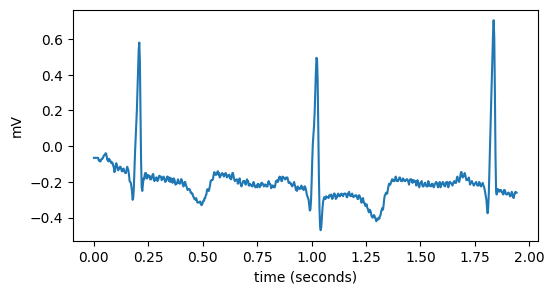
\includegraphics[width=0.7\linewidth]{./img/sebelum_prep.png}}
    % 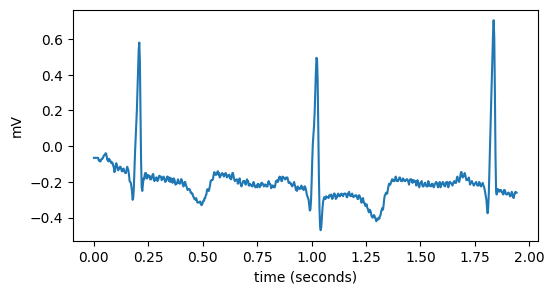
\includegraphics[width=0.6\linewidth]{./img/sebelum_prep.png}
	\caption{Data sebelum \textit{preprocessing}}
	\label{fig:sebelum-prep}
\end{figure}

\begin{figure}[H]
  \centering
  \fbox{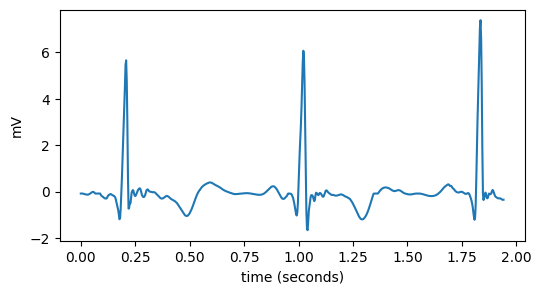
\includegraphics[width=0.7\linewidth]{./img/setelah_prep.png}}
  % 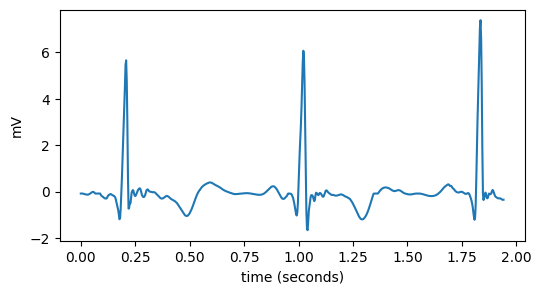
\includegraphics[width=0.6\linewidth]{./img/setelah_prep.png}
  \caption{Data setelah \textit{preprocessing}}
  \label{fig:setelah-prep}
\end{figure}


% Gambar \ref{fig:sebelum-prep} menunjukkan data sebelum dilakukan \textit{preprocessing}, sedangkan Gambar \ref{fig:setelah-prep} menunjukkan data setelah dilakukan \textit{preprocressing}.
Gambar \ref{fig:sebelum-prep} dan \ref{fig:setelah-prep} memperlihatkan perbandingan data ECG sebelum dan setelah dilakukan \textit{preprocessing}.
% Pada Gambar \ref{fig:sebelum-prep}, terlihat bahwa terdapat \textit{noise} berfrekuensi tinggi dan variasi pada \textit{baseline} sinyal ECG.
Pada Gambar \ref{fig:sebelum-prep}, terlihat bahwa pada data ECG masih terdapat gangguan seperti \textit{noise} berfrekuensi tinggi dan variasi pada \textit{baseline} sinyal.
% Setelah dilakukan \textit{preprocessing}, sinyal ECG menjadi lebih halus dan memiliki baseline yang lebih rata.
Setelah dilakukan \textit{preprocessing}, sinyal ECG menjadi lebih halus dan memiliki \textit{baseline} yang lebih rata, seperti yang terlihat pada Gambar \ref{fig:setelah-prep}.

% ---

% Setelah proses \textit{preprocessing} selesai, dilakukan deteksi R-peak menggunakan algoritma Pan-Tompkins untuk menentukan posisi R-peak pada sinyal ECG.
Setelah proses \textit{preprocessing} selesai, dilakukan deteksi R-peak untuk menentukan posisi R-peak pada sinyal ECG.
Deteksi R-peak dilakukan dengan menggunakan algoritma Pan-Tompkins.
Algoritma Pan-Tompkins adalah algoritma yang digunakan untuk mendeteksi R-peak pada sinyal ECG \parencite{panRealtimeQRSDetection1985}.
% Keluaran dari deteksi R-peak adalah posisi R-peak pada sinyal ECG.
Dari posisi R-peak yang dideteksi, dihitung jarak antar R-peak untuk mendapatkan RR-interval.
RR-Interval ini kemudian diekstraksi menjadi 9 fitur seperti yang telah dijelaskan pada Subbab \ref{subsec: bab4-ekstraksi-fitur}.
Fitur-fitur ini kemudian digunakan sebagai input untuk model yang telah dilatih sebelumnya.
Aplikasi web akan melakukan prediksi menggunakan model yang telah dilatih sebelumnya dan menampilkan hasil prediksi pada pengguna.


\section{Pengujian Performa Inferensi}
% pengujian dilakukan dengan cara menghitung waktu inferensi dan memory usage
% pengujian dilakukan dengan menggunakan dataset ecg dengan panjang 10 detik sejumlah 5 kali, panjang 1 menit sejumlah 5 kali, dan panjang 10 menit sejumlah 5 kali
% dari masing-masing 5 kali pengujian, diambil rata-rata waktu inferensi dan memory usage
% pengujian dilakukan pada raspi4 dan intel nuc
% hasil pengujian waktu inferensi dan memory usage akan dibandingkan antara raspi5 dan intel nuc
Pengujian performa inferensi dilakukan untuk mengevaluasi efisiensi dan performa model dalam melakukan inferensi.
Pengujian performa inferensi dilakukan dengan menghitung waktu inferensi dan penggunaan memori yang digunakan oleh aplikasi saat melakukan inferensi.
Waktu inferensi dihitung dari saat aplikasi menerima file rekaman ECG hingga menghasilkan output prediksi.
Penggunaan memori dihitung dari memori maksimum yang digunakan oleh aplikasi saat melakukan inferensi.

Pengujian dilakukan pada dua perangkat tepi, yaitu Raspberry Pi 4 Model B dan Intel NUC.
% Raspberry Pi 4 Model B dilengkapi dengan prosesor ARM Cortex-A72 4-core 1.8 GHz dan RAM 8 GB LPDDR4.
Raspberry Pi 4 Model B yang digunakan pada penelitian ini dilengkapi dengan prosesor ARM Cortex-A72 4-core 1.8 GHz dan RAM 8 GB LPDDR4.
% Sementara itu, Intel NUC menggunakan prosesor Intel Core i3-1115G4 2-core 4-thread 4.1 GHz dan RAM 16 GB DDR4.
Sementara itu, Intel NUC yang digunakan pada penelitian ini dilengkapi dengan prosesor Intel Core i3-1115G4 2-core 4-thread 4.1 GHz dan RAM 16 GB DDR4.
Pada perangkat Raspberry Pi 4 Model B, sistem operasi yang digunakan adalah Raspberry Pi OS Lite, sedangkan pada Intel NUC, sistem operasi yang digunakan adalah Debian yang berjalan pada Windows Subsystem for Linux (WSL).
% Kedua perangkat ini memiliki spesifikasi yang berbeda terutama pada arsitektur prosesor.
% Raspberry Pi 4 Model B menggunakan arsitektur ARM sementara Intel NUC menggunakan arsitektur x86.
% Pengujian pada dua perangkat ini dapat memberikan gambaran kinerja aplikasi pada perangkat dengan arsitektur dan spesifikasi yang berbeda.

Pengujian dilakukan dengan tiga skenario, yaitu pengujian dengan data ECG berdurasi 10 detik, 1 menit, dan 10 menit. 
Pada masing-masing skenario, dilakukan pengujian sebanyak lima kali dengan menggunakan data ECG yang berbeda.
Dari masing-masing lima kali pengujian, diambil rata-rata waktu inferensi dan rata-rata penggunaan memori maksimum.
Hasil pengujian ini akan digunakan untuk mengevaluasi efisiensi dan performa aplikasi dalam melakukan inferensi pada kedua perangkat.
% Masing-masing skenario diulang sebanyak lima kali untuk mendapatkan hasil yang konsisten.
% Dari setiap lima kali pengujian, diambil rata-rata waktu inferensi dan rata-rata penggunaan memori maksimum. 
% Hasil pengujian ini akan digunakan untuk mengevaluasi efisiensi dan performa aplikasi dalam melakukan inferensi pada kedua perangkat.
%
